\chapter{Case-studie: Avstandsoppfølging i Trondheim kommune}
\label{ch:case}

\section{Bakgrunn og tjenesteforløp}
\blindtext

\section{Eksisterende løsning}
Brukeren har et nettbrett som kjører en androidapplikasjon. Denne applikasjonen pakker inn
et webgrensesnitt. I tillegg til hovedapplikasjonen er det en sensorhub-applikasjon som kjører i bakgrunnen
og har ansvaret for tilkoblingen til alle sensorene. Alle skjermbildene i dette delkapittelet er tatt i testmiljøet
til Trondheim kommune i en nettleser.

Beskrivelsen av løsningen og skjermbildene tar utgangspunkt i to scenarioer for sluttbrukere
og ett scenario for helsepersonell: for brukere er det å rapportere dagsform og utføre en måling med pulsoksimeter,
og for helsepersonell er det å gå inn for å se på hvilken data som er kommet inn.

Det første som møter brukeren er hovedskjermen i figur \ref{fig:helsami_hovedskjerm}. I testmodus er alle de ulike
alternativene vist.
Herfra kan brukeren trykke seg inn for å rapportere dagsform for \textit{KOLS} og \textit{HJERTESVIKT}, eller utføre en sensormåling med
enten vekt, blodtrykk eller pulsoksimeter. Det er også mulig å gå på \textit{Brukerveiledninger} for å få instruksjoner og hjelp.
For en bruker som har KOLS og en sensor utplassert hjemme, vil skjermen for eksempel vise KOLS og SpO2.

\begin{figure}
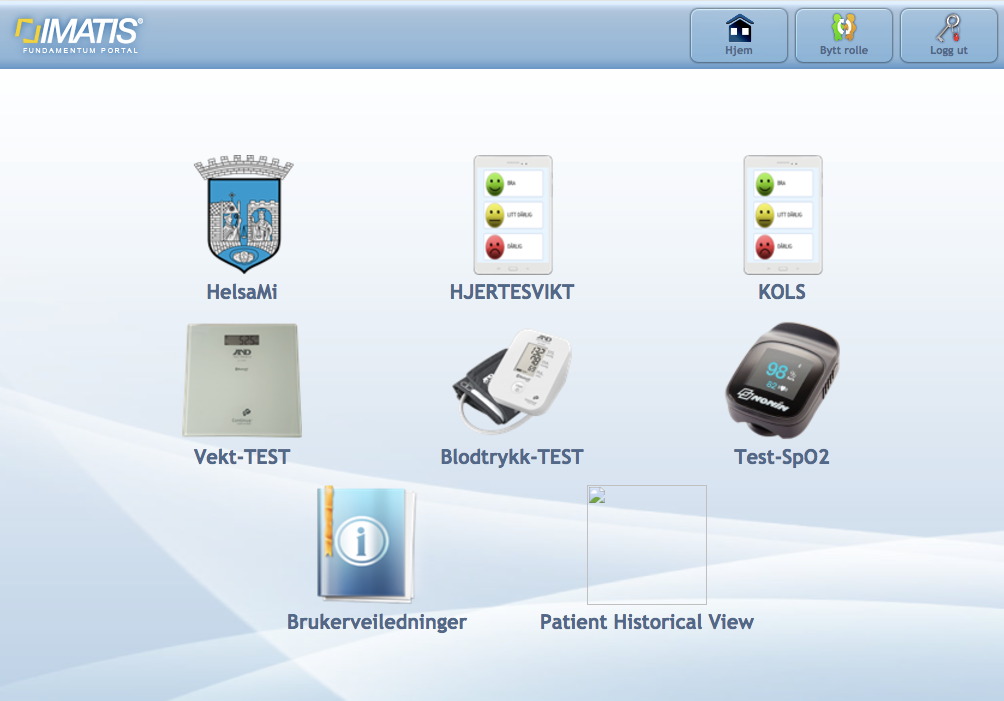
\includegraphics[width=1.0\textwidth,center]{fig/helsami/hovedskjerm}
\caption{HelsaMi+: Hovedskjerm}
\label{fig:helsami_hovedskjerm}
\end{figure}

\subsection{Rapportere dagsform}
Scenariet er at en bruker med KOLS skal rapportere dagsform. Brukeren trykker på KOLS på hovedskjermen,
og kommer til figur \ref{fig:helsami_kols_start}. Et klikk på \textit{Start} tar brukeren til \ref{fig:helsami_kols_sp1}.
Det er fire spørsmål brukeren svarer på. Alle svaralternativer som er subjektive spør brukeren om å sammenligne med
hvordan det er til vanlig.

\begin{itemize}
  \tightlist
  \item Hvordan er pusten din?
  \item Hvordan er hosten?
  \item Hvordan er fargen på oppspyttet ditt?
  \item Hvordan føler du deg til sinns?
\end{itemize}

Etter spørsmålene får brukeren mulighet til å legge inn en skriftlig kommentar og se over at det er greit
før alt sendes inn (figur \ref{fig:helsami_kols_sammendrag}). Brukeren får beskjed om at tilbakemeldingen er sendt,
og må selv aktivt klikke seg tilbake til menyen etterpå.

\begin{figure}
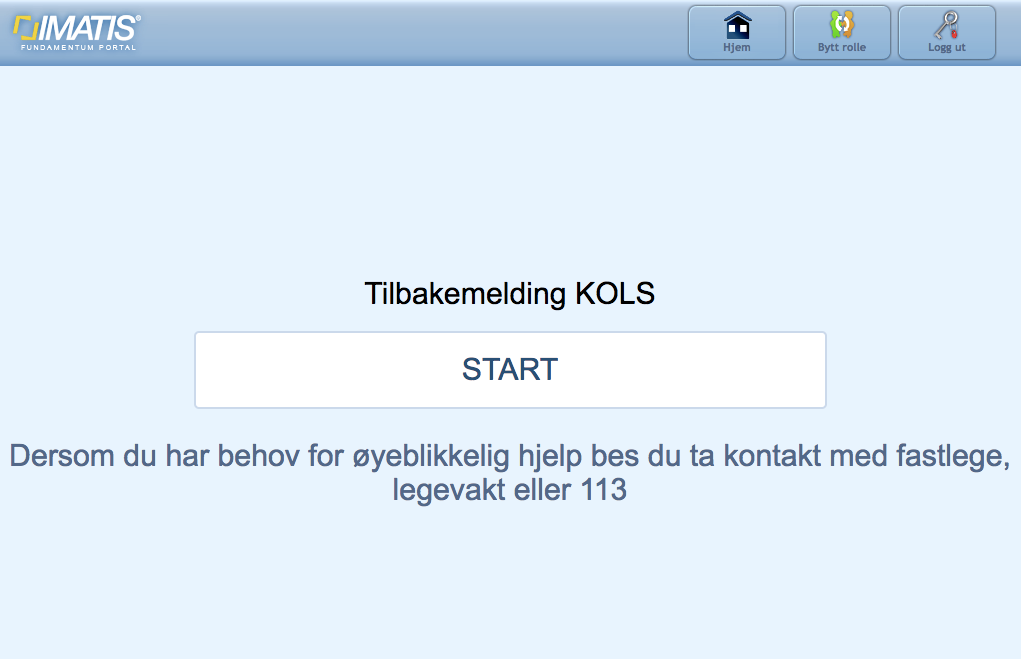
\includegraphics[width=1.0\textwidth,center]{fig/helsami/kols_start}
\caption{HelsaMi+: Tilbakemelding KOLS}
\label{fig:helsami_kols_start}
\end{figure}

\begin{figure}
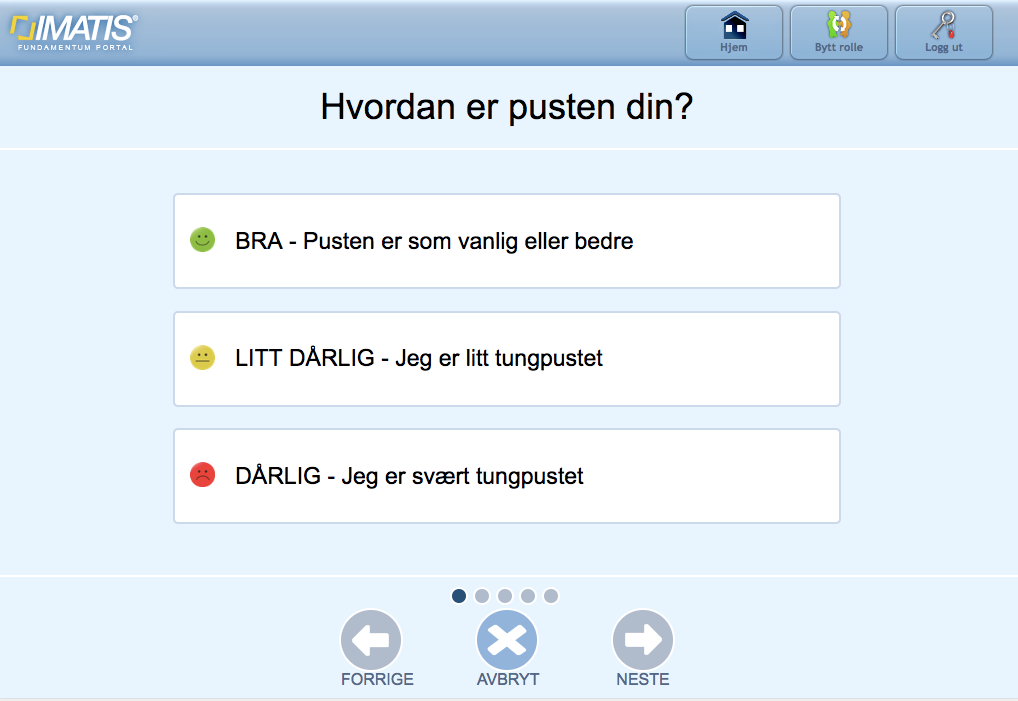
\includegraphics[width=1.0\textwidth,center]{fig/helsami/kols_sp1}
\caption{HelsaMi+: Spørsmål 1}
\label{fig:helsami_kols_sp1}
\end{figure}

\begin{figure}
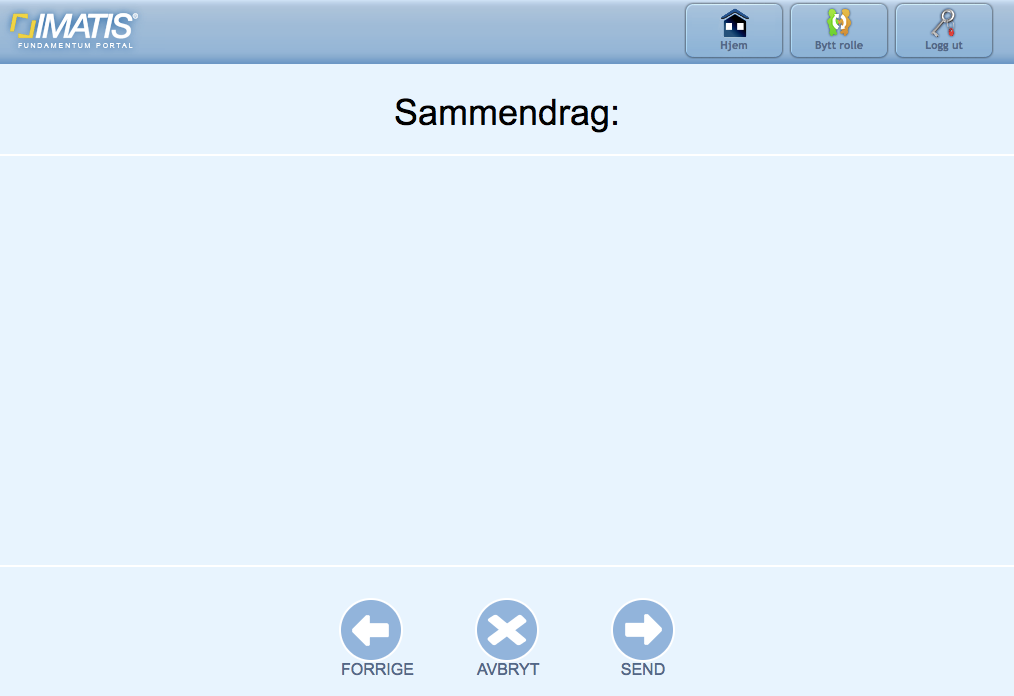
\includegraphics[width=1.0\textwidth,center]{fig/helsami/kols_sammendrag}
\caption{HelsaMi+: Sammendrag}
\label{fig:helsami_kols_sammendrag}
\end{figure}

\subsection{Utføre en måling med pulsoksimeter}
Et klikk på \textit{Test-SpO2} tar brukeren til en mellomskjerm med informasjon om at
brukeren ikke har utført en måling ennå med et bilde av sensoren. Brukeren klikker seg videre
til en skjerm med to valg, enten \textit{Trykk her for å måle oksygenmetning og puls} eller \textit{Trykk her for brukerveiledning}
(figur \ref{fig:helsami_pulsoksimeter_oversikt}). Det første valget tar brukeren til figur \ref{fig:helsami_pulsoksimeter_maaling}
der brukeren klikke på en knapp og setter måleren på fingeren. Brukeren må ha en gyldig sensorhub installert for
å få lov til å gjennomføre en måling.

\begin{figure}
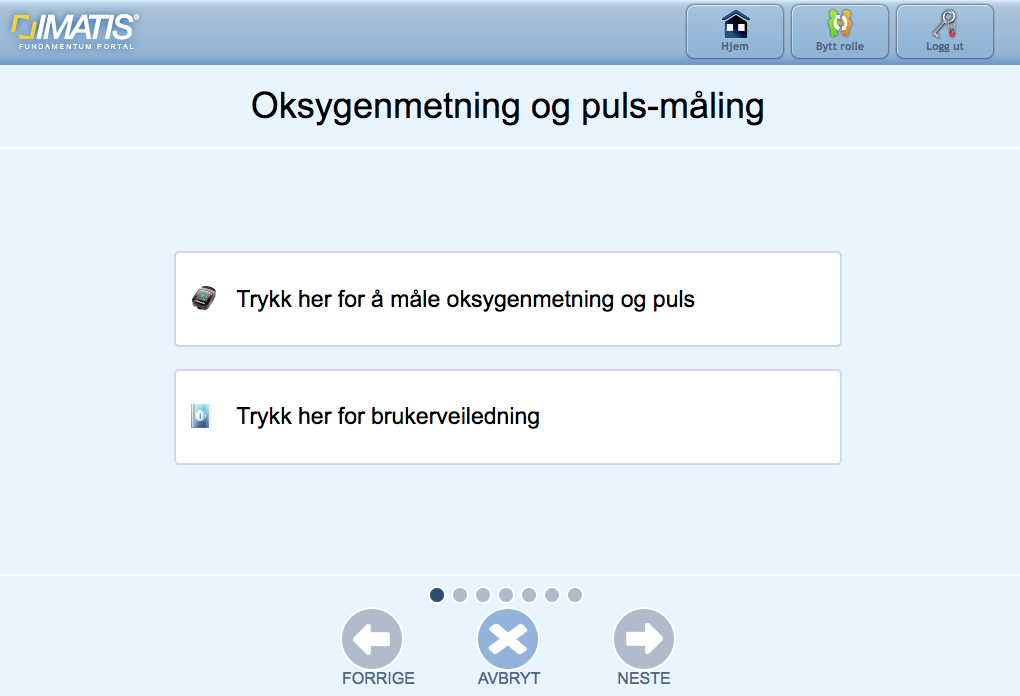
\includegraphics[width=1.0\textwidth,center]{fig/helsami/pulsoksimeter_oversikt}
\caption{HelsaMi+: Pulsoksimeter-oversikt}
\label{fig:helsami_pulsoksimeter_oversikt}
\end{figure}

\begin{figure}
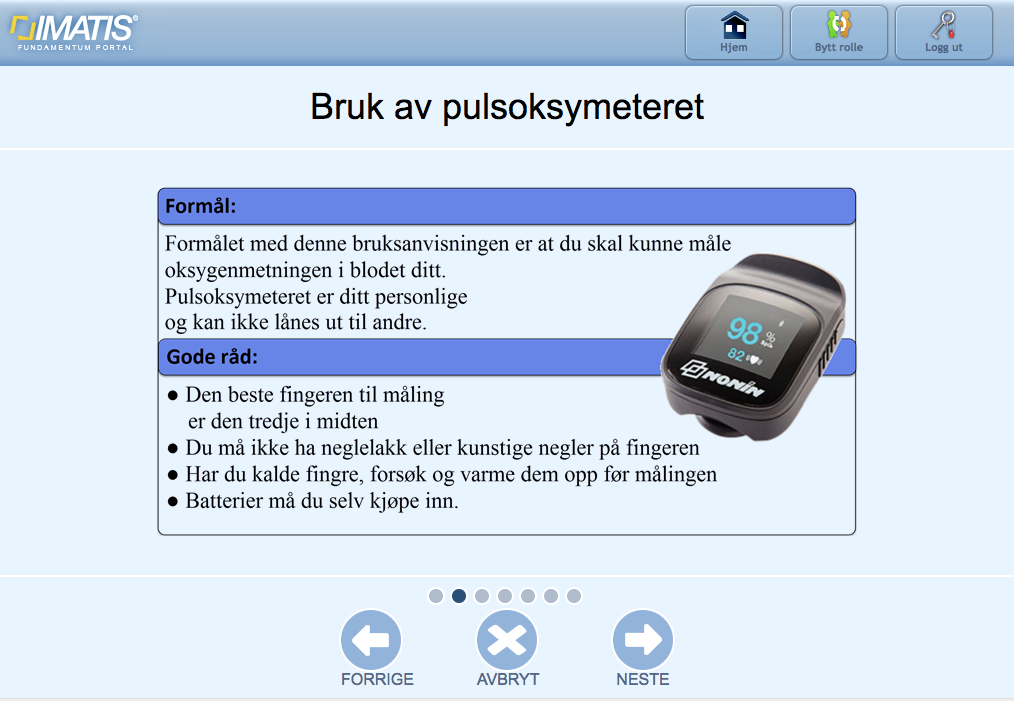
\includegraphics[width=1.0\textwidth,center]{fig/helsami/pulsoksimeter_veiledning}
\caption{Pulsoksimeter-veiledning}
\label{fig:helsami_pulsoksimeter_veiledning}
\end{figure}

\begin{figure}
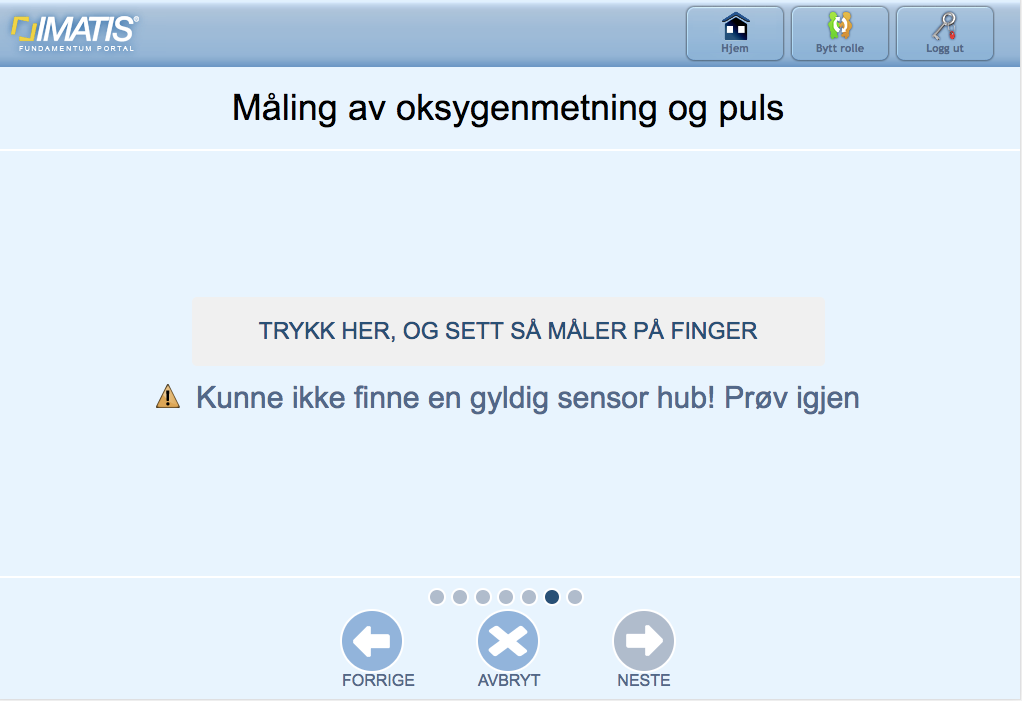
\includegraphics[width=1.0\textwidth,center]{fig/helsami/pulsoksimeter_maaling}
\caption{HelsaMi+: Pulsoksimeter-måleskjerm}
\label{fig:helsami_pulsoksimeter_maaling}
\end{figure}

\subsection{Se på innrapport data}
Trykk på \textit{HelsaMi}. Figur \ref{fig:helsami_admin1} viser hvordan oversikten over innrapportert data ser ut.

\begin{figure}
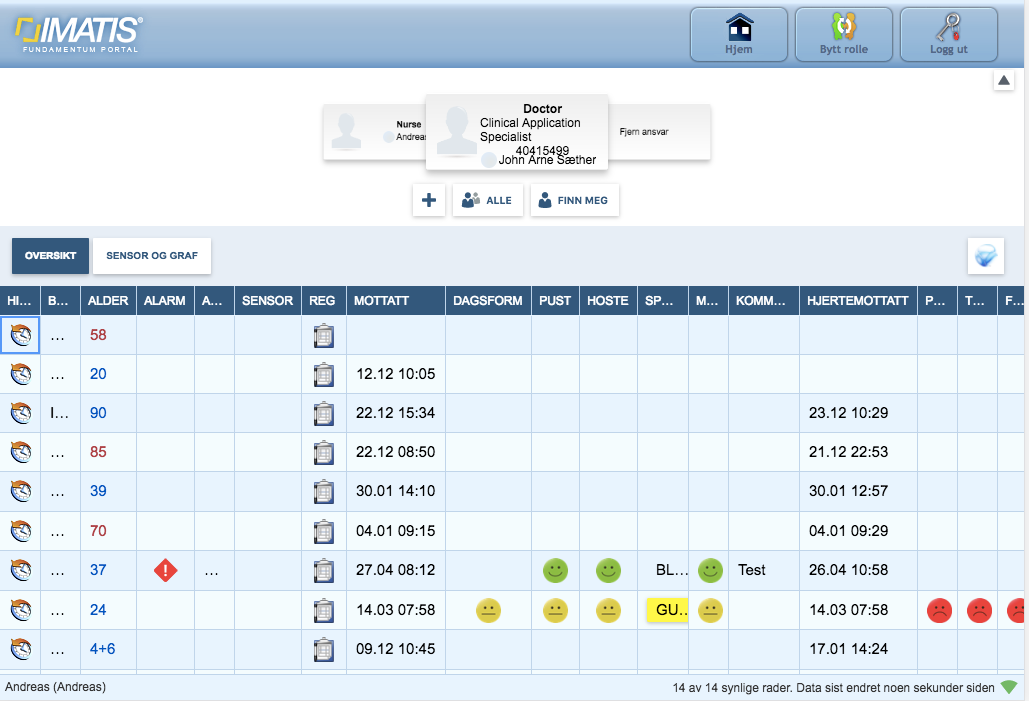
\includegraphics[width=1.0\textwidth,center]{fig/helsami/admin_oversikt}
\caption{HelsaMi+: Oversikt for administrator 1/2}
\label{fig:helsami_admin1}
\end{figure}

\section{Fremtidige planer}
